\documentclass[onecolumn, draftclsnofoot, 10pt, compsoc]{IEEEtran}
\usepackage[margin=0.75in]{geometry}

\usepackage{cite}
\usepackage{graphicx}
\usepackage{setspace}
%\usepackage{tabularx}
%\usepackage{pgfgantt}
\usepackage{listings}
\usepackage{pdfpages}
\usepackage{float}
\usepackage{hyperref}

\hypersetup{
    colorlinks=true,
    linkcolor=blue,
    urlcolor=cyan,
}

\renewcommand{\arraystretch}{1.7}

\newcommand{\hiddensection}[1]{%
  \par\refstepcounter{section}% Increase section counter
  \sectionmark{#1}% Add section mark (header)
  \addcontentsline{toc}{section}{\protect\numberline{\thesection}#1}% Add section to ToC
  % Add more content here, if needed.
}

\newcommand{\hiddensubsection}[1]{%
  \par\refstepcounter{subsection}% Increase section counter
  \subsectionmark{#1}% Add section mark (header)
  \addcontentsline{toc}{subsection}{\protect\numberline{\thesubsection}#1}% Add section to ToC
  % Add more content here, if needed.
}

% 1. Fill in these details
\def \CapstoneTeamName{		Auction Hunter}
\def \CapstoneTeamNumber{		4}
\def \GroupMemberOne{			Alexander Hull}
\def \GroupMemberTwo{			Alexander Jacobson}
\def \GroupMemberThree{			Yufei Zeng}
\def \CapstoneProjectName{		Auction Hunter}
\def \CapstoneSponsorCompany{	}
\def \CapstoneSponsorPerson{		Ryan Kalb}

% 2. Uncomment the appropriate line below so that the document type works
\def \DocType{		%Problem Statement
				%Requirements Document
				%Technology Review
				Final Document
				%Progress Report
				}
			
\newcommand{\NameSigPair}[1]{\par
\makebox[2.75in][r]{#1} \hfil 	\makebox[3.25in]{\makebox[2.25in]{\hrulefill} \hfill		\makebox[.75in]{\hrulefill}}
\par\vspace{-12pt} \textit{\tiny\noindent
\makebox[2.75in]{} \hfil		\makebox[3.25in]{\makebox[2.25in][r]{Signature} \hfill	\makebox[.75in][r]{Date}}}}
% 3. If the document is not to be signed, uncomment the RENEWcommand below
%\renewcommand{\NameSigPair}[1]{#1}

%%%%%%%%%%%%%%%%%%%%%%%%%%%%%%%%%%%%%%%
\begin{document}
\begin{titlepage}
    \pagenumbering{gobble}
    \begin{singlespace}
    	
\includegraphics[height=4cm]{coe_v_spot1}
        \hfill 
        % 4. If you have a logo, use this includegraphics command to put it on the coversheet.
        %\includegraphics[height=4cm]{CompanyLogo}   
        \par\vspace{.2in}
        \centering
        \scshape{
            \huge CS Capstone \DocType \par
            {\large\today}\par
            \vspace{.5in}
            \textbf{\Huge\CapstoneProjectName}\par
            \vfill
            {\large Prepared for}\par
            \Huge \CapstoneSponsorCompany\par
            \vspace{5pt}
            {\Large\NameSigPair{\CapstoneSponsorPerson}\par}
            {\large Prepared by }\par
            Group\CapstoneTeamNumber\par
            % 5. comment out the line below this one if you do not wish to name your team
            \CapstoneTeamName\par 
            \vspace{5pt}
            {\Large
                \NameSigPair{\GroupMemberOne}\par
                \NameSigPair{\GroupMemberTwo}\par
                \NameSigPair{\GroupMemberThree}\par
            }
            \vspace{20pt}
        }
        \begin{abstract}
        % 6. Fill in your abstract    
        	This design document outlines the components of our Auction Hunter development project. The elements, relationships, and design concerns will be discussed for each. This will serve as a road map for the remainder of this project. 
        \end{abstract}     
    \end{singlespace}
\end{titlepage}

\newpage
\tableofcontents
\newpage

\section{Introduction}
Auction Hunter was a project requested by Ryan Kalb, our client. It is meant to improve and exhance a user's experience when searching for salvaged car auctions. If someone totals a vehicle, the car will sometimes be auctioned by insurance companies. Some of these are perfectly fixable but insurance companies opt to sell them due to exorbitant repair costs charged by body shops. 

When implemented, this tool could be used to maximize profits when selling spare parts or rebuilding vehicles. It could also be used by the public to make sure they are getting a good deal. Action Hunter will help users gather data on these cars quickly and conveniently.

\subsection{Members}
\begin{itemize}
    \item Alexander Hull - Worked on database, value calculation, and web scraping.
    \item Alexander Jacobson - Worked on front end development, and managed a server for the. project
    \item Yufei Zeng - Worked on researching and implementing Web Scraping.
    \item Ryan Kalb - Established requirements and provided feedback.
\end{itemize}



\hiddensection{Requirements Document}

\includepdf[pages=-]{Requirements.pdf}

\hiddensection{Design Document}

\includepdf[pages=-]{DesignDocument.pdf}

\hiddensection{Tech Reviews}

\hiddensubsection{Tech Review - Alexander Hull}
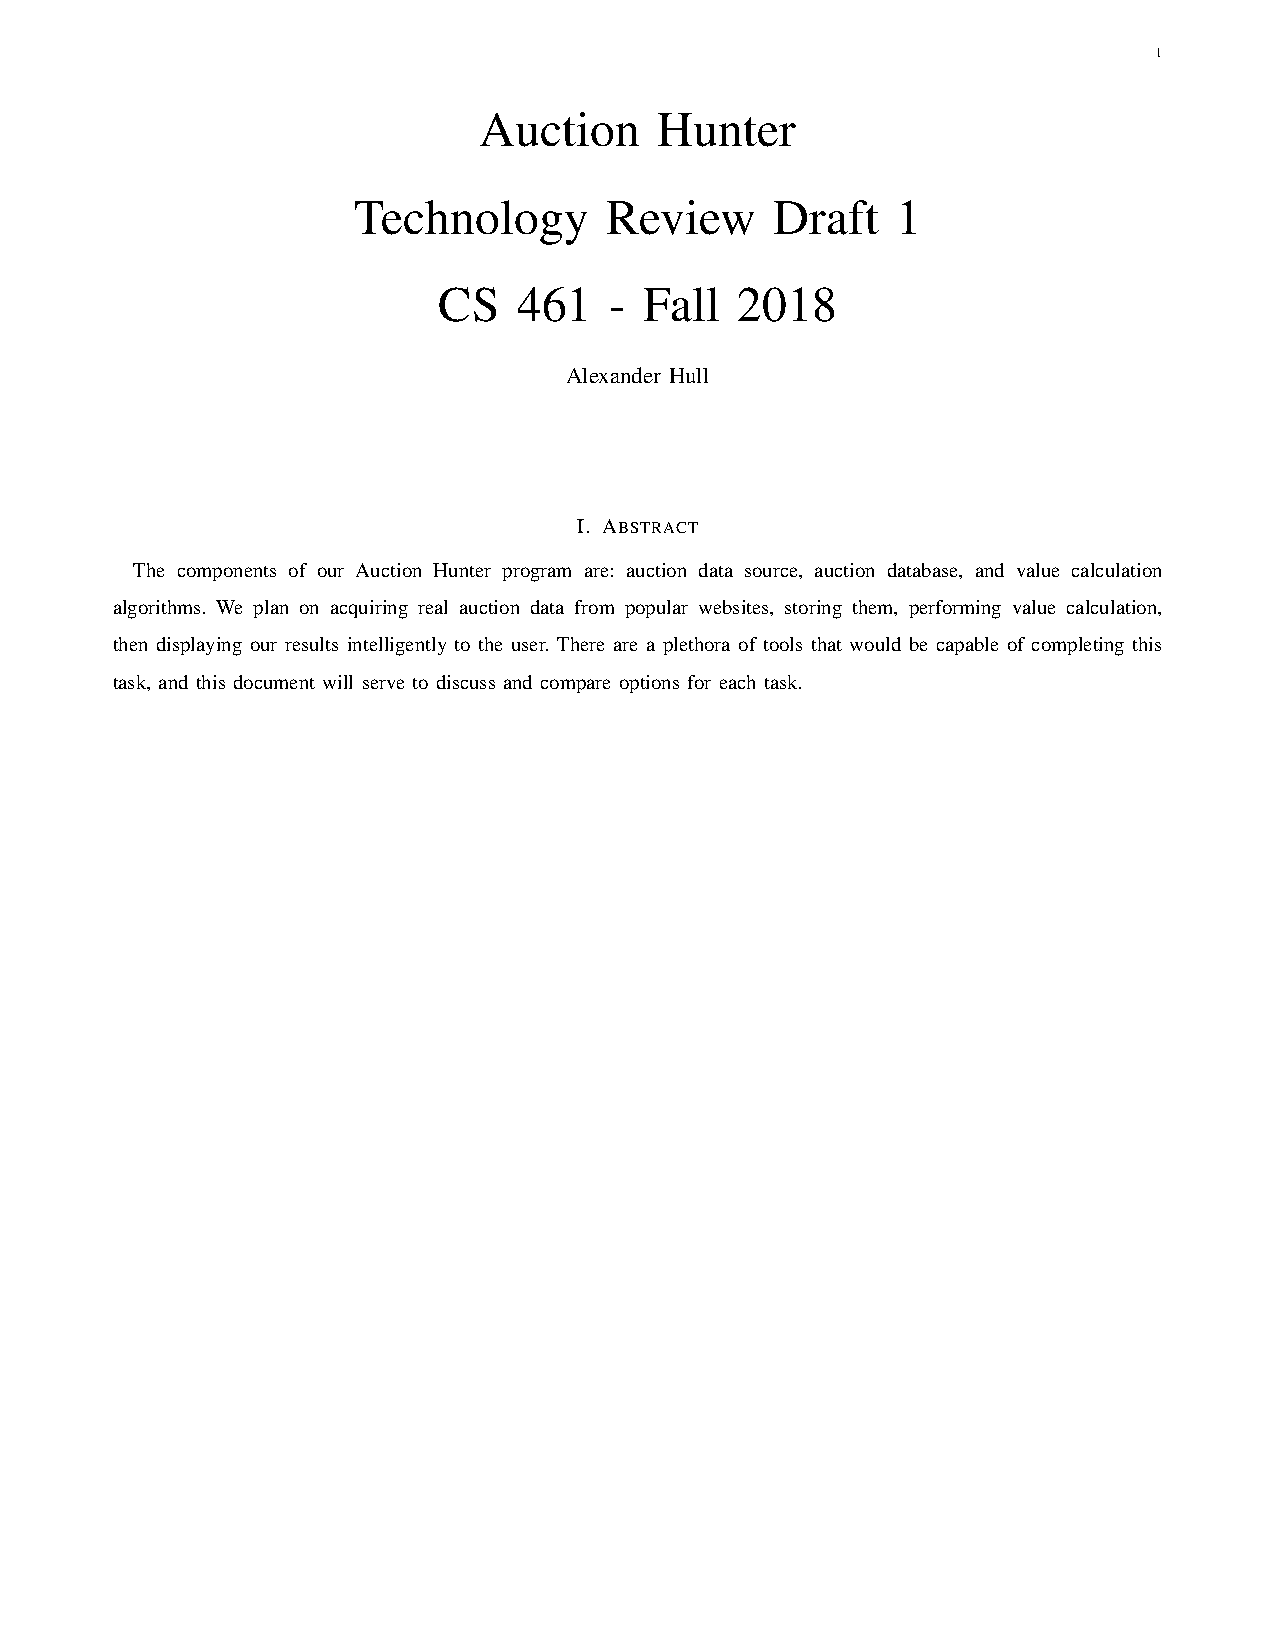
\includepdf[pages=-]{TechReviewHull.pdf}

\hiddensubsection{Tech Review - Alex Jacobson}

\includepdf[pages=-]{TechReviewJacobson.pdf}

\hiddensubsection{Tech Review - Yufei Zeng}

\includepdf[pages=-]{TechReviewZeng.pdf}

\section{Weekly Blog Posts}
\subsection{Alex Hull}
\subsubsection{Fall}
 
\textbf{Week 4:}
I have learned a bit more about using LaTeX. I started using overleaf which is significantly easier for quick drafting and viewing changes immediately. I learned in a different class how to use a Makefile for LaTeX as well. I finished my problem statement, and I'm currently working on finishing the group problem statement.
I plan to complete the group problem statement tonight. I also want to look into other forms of communication so my group can collaborate on a project at the same time while working remotely.
\newline
\textbf{Week 5:}
Our team has drafted up the majority of our requirements document. We are now waiting to hear back from our client to get some feedback and/or approval. 
We plan to complete the requirements document this weekend, after we hear back from our client. 
\newline
\textbf{Week 6:}
Our group recently finished the requirements document. I think we collaborated well for this last assignment and things went well. Our group also got together and assigned portions of the project for the tech review.
I plan to complete the tech review today and then enjoy my weekend. 
\newline
\textbf{Week 7:}
I am working on applying all feedback from the tech review peer review. I am nearly complete, I just need to make a few final changes. 
I am struggling to find relevant and useful citations for my tech review. There aren't too many unbiased discussion comparing the technologies I'm working with. If I go to the MongoDB website, I can only find positive commentary about their product. 
I plan to finish up my tech review today. 
\newline
\textbf{Week 8:}
Our group has not had very much work to do for our project the last week. One thing I have been working on is getting in better contact with our TA. I have contacted Kirsten Winters with this issue and she has met with the TA. 
We are running into a problem where it is difficult to get into contact with our TA. We haven't had anything graded yet and we want to make sure that we have met with our TA to go over anything that he ends up grading. 
I plan to wait a couple more days to give our TA a chance to respond to my message, and a chance to grade our papers. If I find that neither of these are completed, I will have to contact the TA and Kirsten again until it is resolved. 
\newline
\textbf{Week 9:}
We still haven't heard back from our TA, although Kirsten Winters has communicated with us on his behalf. 
We plan to begin working on the design document soon. Since we are all celebrating the holiday weekend, we likely won't putting a lot of work into it until the Sunday. Thankfully there are large individual components that we can all think about before starting. 

\subsubsection{Winter}
\textbf{Week 1}
Our group has begun to get back into the swing of things. We are organizing a time for us to meet with our TA, and made sure that everyone can make the required class time.
One problem I have is I may have a scheduling conflict with our required class time. I am hoping that there isn't a conflict, and I'm continually checking my other event to make sure it doesn't conflict. 
Our group plans to meet on a more regular basis with our TA than we were used to the previous term. We are starting to think about implementation and how to delegate sub tasks. 
\newline
\textbf{Week 2}
We have met with out TA, and once with just our group. We have set up a server for us to develop and test code on, and organized out GitHub repo a bit so we all know where to keep our code. We have roughly divided up the tasks for who will manage each part of the project. Once we feel a good prototype is finished, we can reevaluate and plan for future development. 
 We are not entirely sure of deadlines that we are planning on meeting.  
We plan to all work individually on our components. We will be working on the poster and elevator speech in the coming weekend. 
\newline
\textbf{Week 3}
I have personally finished a good starter code for our database component of our project. I created a pull request to be viewed by my teammates. Hopefully this will be useful for them to base their own development off of.
One issue I had this week was I forgot to go to our meeting with our TA. I was able to communicate with my team over slack to get all the details from the meeting. 
I plan to continue perfecting my database component, to make to easier to combine with the other components. Currently, there is a main() function which tests out the other functions that I implemented. I will need to eventually remove the main function so that other python files can call my functions.
\newline
\textbf{Week 4}
Made pull request for starting database code. Completed the elevator speech session with group. 
I plan to create a more concrete plan in terms of implementation due dates. Hopefully this will allow us to avoid procrastination. 
\newline
\textbf{Week 5}
We have been individually working on our components and have agreed to begin tying together the pieces in the coming week. 
Our group will plan on piecing together an alpha version of our project by the end of week 6. We are presumably working on midterms at this time so finding time to work could be difficult. 
\newline
\textbf{Week 6}
Our group has all made individual progress on our components. We completed the poster review, and now have some good notes of pieces to change. 
We plan to put all the pieces together to create an alpha version over the weekend. Since the progress report has been pushed back a week, it allows us to spend more time putting together the alpha version.
\newline
\textbf{Week 7}
We are collectively working on getting our alpha version up and running. 
We plan to meet this weekend to finalize our alpha and work on the progress report that is due on Monday. I suspect that this will be a multiple day endeavor.
\newline
\textbf{Week 8}
We were able to get together as a group and connect the individual components that we have been working on. We are able to pull information off the websites, store it in the database, then display through a web interface. Now, improving each step of the process will be relatively easy, and also simple to test. 
Haven't had any major problems this week. One 'problem' is a lot of my initial work on the database side ended up being pointless because our scraper, mongodb and web side all interface with each other by default. However, the work I did should make it easier to add some additional complex queries or updates. 
We plan to improve the UI, and increase the amount of information we provide on each car. I am also planning on creating some rudimentary value prediction algorithms to start displaying and being able to sort on.
\newline
\textbf{Week 9}
One problem that we had was that I was sick so I wasn't able to attend the TA meeting. 
We plan to work on the progress report and our project in the coming week. I personally have less work than normal in the coming week so I should be able to allocate a lot of time to our project. 
\newline
\textbf{Week 10}
We have begun to work on the data acquisition and auction ranking. Once we put that together we should have a complete beta.
No major problems to speak of, other than balancing this project and other classes.
We plan to work a lot on the project over the weekend, then work on the progress report and video once we have reached a beta point on the project.

\subsubsection{Spring}

\textbf{Week 1}
I am starting to work the web scraping, because I think it is one of the more difficult components, and it is a precursor to my database work. Previously we were scraping a single page and we were only getting data from the preview. I'm working on making it so the scraper actually follows the links and goes through all the pages. This will make our data a lot more robust and we will have more of it. 
I plan to organize a schedule for us to finish up the project before the code freeze at our TA meeting today. 
\newline
\textbf{Week 2}
I have been working on enhancing our scraper to also get pricing information from the website. This has been especially difficult because instead of getting all our info from one web page, we actually have to follow links and back out. I also found that the VIN information has been masked on the web page, which makes scraping it difficult. I think they did this to prevent what I am doing. Another problem is the website uses javascript to handle the next page button, instead of a simple link. This is also very difficult to scrape and follow the link. 
I plan to finish up this task, then make sure our project is ready to go. We will also have to provide instructions to build and run. 
\newline
\textbf{Week 3}
We submitted the code review, and I starting work on getting the revisions emailed to our client for verification. 
I just finished the confirmation of the EXPO details assignment. 
\newline
\textbf{Week 4}
We are currently working on our poster. I was able to keep notes from the poster review, so I am starting with applying those changes. I am still trying to get our client to verify our design document and requirements document. 
I attended one of the required speakers last Friday, so I only have to worry about the poster and expo for the coming weeks. 
\newline
\textbf{Week 5}
We have finished submitting our poster. We had to make some last minute changes to make sure there was a picture of us and there were captions. 
I am still having difficulty getting our client to verify our design and requirement documents. It seems that he is very busy, and also might be disappointed that we didn't finish the stretch goals that we had established at the beginning. In hindsight, we had a lot of lofty goals for our project that were unrealistic. We also didn't establish an open thread of communication with our client, so we were unaware of his plans for the project, and he was unaware of our progress. 
We plan to talk more with our client to see if we can get this resolved, and if there is any additional work we can put into the project that he would like to see. 
\newline
\textbf{Week 6}
Our group is trying to meet to discuss what we are going to present for expo. We are discussing whether we are going to have a monitor displaying the front end, or possibly the back end components. 
I still need to meet with Kirsten to ask her if we are allowed to show anything at expo that wasn't done by us. Since we have an active pull request for an update to our front-end by somebody unaffiliated with our group. 


\subsection{Alexander Jacobson}
\subsubsection{Fall}
\textbf{Week 4}
This week I worked on combining the individual problem statements into a group version. We haven't had many problems, our client responds promptly, and we are able to stay pretty organized by using slack and discord to group voice chat. Our plan for next week is to work on our requirements document and talk to our client about our problem statements. 
\newline
\textbf{Week 5}
This week I worked on the requirements document with the team. We haven't been meeting in person, mostly just on discord which has been working well for us. Our client has been a little busy so we haven't gotten as much feedback as expected but I'm confident we understand what our client wants and can articulate it onto the page. Plan for next week is to finish the requirements document and design who is going to take which parts for the tech review. 
\newline
\textbf{Week 6}
This week my group figured out our requirements for our project. This was mostly painless except for getting everyone working on the same latex document can be a pain. We submitted our draft for the specification buts for our final one our stakeholder suggested some changes which we will make. We also had the tech assignment this week which was hard because we had to come up with 9 different things for people to research. Once we got that all sorted out it wasn't much of an issue to write. Next week is our final version of the tech paper is due so I will need to work on that. We also have a midterm sometime so need to figure out what that's about.
\newline
\textbf{Week 7}
We didn't do a lot as a group this week because we are focusing on our tech reviews which the final version is due on Friday night. So no group progress or problems to report. It doesn't look like we have anything due till the 27th, but that assignment looks quite large, so we will need to meet as a group and plan out how to tackle it. Once we distribute some of the work, we can meet again at the end of the week for a progress update. 
\newline
\textbf{Week 8}
We finished the tech review final version this week. I had broken my collarbone a couple of weeks back so it has been difficult to type, so I turned my tech review in late. Not sure what we as a team are going to do next week, but I am researching potential tools and designs to use for our implementation phase of the project. 
\newline
\textbf{Week 9}
We worked on design document by taking all of our individual parts from our respective tech reviews and compiling them together. It turns out that we probably should have coordinated a little better on our tech reviews because some of our individual choices didn't make sense when we put them together with the rest of the project. We are working on the video and final progress update this weekend and next week.
\subsubsection{Winter}
\textbf{Week 1}
This I setup our development server and build tools so that we could get started developing as soon as possible. We still need to do some more organisation and timelining exactly when each part needs to be done, but so far so good. My group needs to spend some more time planning our term out, but we can resolve that this weekend. 
\newline
\textbf{Week 2}
This week we worked on planning as a group to figure out what we need to do individually. I then worked on setting up a prototype of what the front end website will look like, and begun building the tool chain to run it. I've also started working on automating the build and deploy tools so that we can focus on developing and not hitting the deploy button a million times. Next week we are going to work on the poster and our elevator speech.
\newline
\textbf{Week 3}
This week I worked on getting the build system working. So I can now run two commands that my website back-end and front-end both get built and deployed on a local computer. This isn't quite working for a full production deployment, but that should be soon to come. This also works on the server I have hosted. I can now access an example version of the website remotely hosted off the server. Next week I am going to be working on getting the skeleton of the front-end in place to then build out.
\newline
\textbf{Week 4}
This past week I finished with the skeleton of the front-end and now I am going to work on getting each page of the site laid out with fake data to make sure it looks nice and will support all the features needed. There are quite a few different pages, login screen (w/ error messages), home page, detail page, account page, etc...
\newline
\textbf{Week 5}
Got most of the individual pages laid out and filled with temp data. Haven't finished them all so that will be a bit of work this week too. After that I am going to work on getting the back-end REST API setup so I can start reading data from the database into the front-end. I probably won't get any individual pages working, just the whole consuming pipeline working.
\newline
\textbf{Week 6}
Got the REST API working on the back-end. Having trouble creating a standard front-end consumer pipeline though. I don't have any of the individual pages working, but once I have the pipeline in place I can will get some of the basic page data into the home page and maybe a details page.
\newline
\textbf{Week 7}
This past week I got the home page working. So it lists basic data and links to an image of the vehicle. I have a standard way of receiving data from the back-end, but I realized that I am also going to to have to send some data as well from the front-end back to the back-end. So next week is getting sending from the front-end to the back-end working and also getting the details page populated with correct data from the back-end.
\newline
\textbf{Week 8}
Sending data is turning out to be kind of difficult with authentication and everything, but I have something hacked together working now. I didn't get the details pages working yet, that will be for next week. I also going to soon need to start integrating with the crawler and the database more directly. We need to be able to get as much data from the external sites as possible, so I can display it all in the front-end details page.
\newline
\textbf{Week 9}
Got the details pages worked out fairly well. It seems like we have more information from the crawler progress so that's good. Now I need to work on the user account page some more as well as making sure I can interact with the site effectively (i.e. clicking on a row gives you a detail of the car, the pictures load all correctly, malformed data is handled correctly, etc.).
\newline
\textbf{Week 10}
Got the user account page working (mostly) and so users can login and set alerts for types of cars. Nothing is going to send the alert yet, but that's almost done. I have a mostly feature complete front-end and the database has most of the data we will need. Will probably try and clean it up in the future to make it so we don't have strange corner cases appearing in the details page.
\subsubsection{Spring}
\textbf{Week 1}
Right now we are in the final push to clean everything up and write the build scripts to make it easy to run. This week I mostly focused on packaging my code for "production" vs. "development". This means changing a bunch of flags in my normal scripts and finding a fully fledged hosting solution rather than just the built in web server that Django has. Most of my issues have revolved around getting the new web server working. Next week we are going to work on getting out clients approval on everything and fixing any issues or bugs that he finds.
\newline
\textbf{Week 2}
Worked on fixing all the bugs so demo runs without a problem. Still need to write the directions for running the code. Not really any problems other than just lack of time. Never enough hours in the day (yes planning ahead would help alleviate this). We are going to finish everything up for the demo this weekend then work on the document revision next week before its due next Friday I believe. 
\newline
\textbf{Week 3}
This week I worked on documentation for the code, and getting approval for our modified requirements document. We had some trouble getting the whole team getting everyone in the same place (virtual or otherwise), but eventually got it organized. Next week we have the poster due which we are going to work on, before Friday.
\newline
\textbf{Week 4}
This week I worked on the poster with the team. I accidentally missed the meeting where we were going to finalize it, but I reconnected with them later and we finished it all up before it was due. Not sure what else I need to work on for this. I have been adding little features to our site over time to make it better for expo, but other than that unsure what to improve.
\newline
\textbf{Week 5}
This week we got our poster done expo is coming up. Still some tweaking and other things we need to do for the project before expo. We also need to get our client to verify our stuff. I've been messaging him, but he hasn't taken a look at our stuff yet.  He doesn't seem super please with what we got, but also I wish we got more done too. Next week is figuring out expo stuff and client verification.
\newline
\textbf{Week 6}
Not much progress this week. Haven't really talked to the team either, we have been setting up meetings and all bailing on them. Not much else other than picking who is going to be where and when for expo, and what exactly we want to show off.
\subsection{Yufei Zeng}
\subsubsection{Fall}
\textbf{Week 4}
We were working on requirements document. And my role is to write the performance requirement.The problem is that We don’t know how web crawler will work at this time. We were going to meet next week for Tech Review.
\newline
\textbf{Week 5}
I and my group was working on group problem statement this week.We exchange the idea for our project from each one's paper.One of our group member has a bone fracture. So we were using discord to discuss. The problem is that We are still waiting for the response from client for user story part. It is hard to distinguish the project with other common used-car side. We need some more notable features to attract users. We are going to meet again at Sunday for requirements document.
We are going to see TA next week for next step.
\newline
\textbf{Week 6}
I met my group this Wednesday. We have assigned work for each person for Tech Review.  Alex Hull is responsible for database choice, auction ranking system and where to pull auction data form.  Alex Jacobson is responsible for website: coding language / framework, hosting solution and build system. I'm responsible for crawler: coding language / framework, damage estimation engine, and code repository / collaboration software. The problem we met is that we don't know if the assigned work fits each other, and if they can finish their work well. So we might change the position later. We are going to meet again on next week Monday through discord to talk about more project.
\newline
\textbf{Week 7}
I have done a Tech review peer review this week during class activity. During this event, we exchange ideas each other. I found many good ideas, and I have learned much about how to write a Tech review  follow IEEE format. My project group didn't meet this week. Because all of work we are doing is individual. I don't know their progress. I don't know if my the techonology in my tech review fits the project. I look forward next meeting. I will meet with my group next Sunday maybe for design document.  And I will continue to know more about the contents on Tech review.
\newline
\textbf{Week 8}
We were working on  Tech review last week, and we have assigned the task to everyone.  Alex J is responsible for website: coding language / framework and  hosting solution. Alex H is responsible for database choice, auction ranking system, and where to pull auction data from. I'm responsible for crawler: coding language / framework, damage estimation engine, and code repository / collaboration software.We don't know if the assigned work fits everyone well. So we still need some time to think about this.We are going to meet and work on Design document draft next week.
\newline
\textbf{Week 9}
I'm working on my individual work for Design Document: Draft 1. I'm trying to add some proper introduction and conclusion for them. So my group can combine them to one document.I think one part of my individual work(damage estimation engine) which is not suitable for me very well. I'm trying to talk this with my teammates. But all good.We are going to meet with our client through Slack next week for verification.
\subsubsection{Winter}
\textbf{Week 1}
We all went back to work this week. I'm working on crawler and damage estimation engine for Auction Hunter. Client askes our team to add a track progress and ticketing system. We are going to talk about this during next meeting. We are going to meet with TA every Wednesday 11.59 AM.
\newline
\textbf{Week 2}
The first meeting has been completed. We have assigned the task to everybody.  I'm responsible for web crawler, Alex Hull is responsible for database, and Alex Jac is responsible for interface. In addition, we have met TA this week, and talk to him about our project. We have to make a detailed schedule for our project. So we can finish each part on time. We are going to meet each Tuesday 6pm, and meet with TA each Wednesday 12pm to talk about the progress.
\newline
\textbf{Week 3}
We are still working on Auction Hunter implement this week. We are using github to share and store the code, and I'm responsible for web crawler part.Web crawler is totally new thing for me, and I'm going to use Scrapy open source tool as the framework. I still need some time to be familiar with it. We are going to have group meeting every Tuesday at 6pm to exchange our research and TA meeting every Wednesday at12pm to talk about project's progress.
\newline
\textbf{Week 4}
This week we have completed Elevator Pitch and Poster. In addition, I'm working on my web crawler part for our project Auction Hunter. The open source web crawler I'm using is Scrapy which are written in Python language.  I still need some time to familiar with this tool.We are going to meet with other group next Friday for Poster Critique Session. And we are going to meet with our TA to talk about our progress next Wednesday 12am.
\newline
\textbf{Week 5}
We have met the other group  for poster critique today. We are still working on project implementing. I'm responsible for web crawler. The prototype of Auction Hunter need to be done on Feb 18. We are on a tight schedule.We are going to have group meeting next Tuesday 6pm, and meet with TA next Wednesday 12am.
\newline
\textbf{Week 6}
I'm still working on my individual part web crawler. I have been able to scrape some basic elements like the names and images of car from a specific website. The next step is to think about what kind of datas we actually needed. Then download these datas to local, and classify or sort them by different scheme. We need some time to put all things together. We are going to have a group meeting next Tuesday 6pm, and meet with TA on Wednesday 12am.
\newline
\textbf{Week 7}
I'm still working on my part web crawler.  I have been able to scrape some basic elements(bidding time, car's images, car's informations) from the specific page, and my spiders can automatically loads to next page of the site. I'm trying to figure out how to download the image through url to local.We are trying to piece together everything.We are going to have a group meeting next Tuesday and demo our project to our TA next Wednesday.  
\newline
\textbf{Week 8}
We are working on improvement our scraping logic. We have been able to intergrade the scraping data into our mongo database this week, but we need more valuable data. We need to figure out how to reconsctruct the scraping data, and make them to be more valuable. We are going to demo our alpha version to our TA next Wednesday, and we have a group meeting on next Tuesday.
\newline
\textbf{Week 9}
We are working on interface and improvement scraping for our auction hunter. We have been able to scrape the necessary elements from specifc website like IAAI, and store the data into our database. We are still looking for a method for implementing damage estimate. We are going to meet with TA next Wednesday, and have a group meeting next Tuesday.
\newline
\textbf{Week 10}
I'm still working on improvement web crawler.  I have been able to scrape some basic elements(bidding time, car's images, car's informations) from the specific page, and my spiders can automatically loads to next page of the site. I'm going to create several spiders for different sources of auction. In addition, the scraped datas have been able to store to our mango database automatically. My teammates are working on interface. We are trying to make the interface being user-friendly, and show everything we got on interface.We are going to have a group meeting and finish our final project video next Tuesday.
\subsubsection{Spring}
\textbf{Week 1}
I'm still working on improvement web crawler.  I have been able to scrape some basic elements(bidding time, car's images, car's informations) from the specific page, and my spiders can automatically loads to next page of the site.  I'm going to create more spiders for different source sites.We are trying to make the interface being user-friendly, and show everything we got on interface. I'm going to attend Charles Shaffer: 4/8-Monday/Presentation at 12:30-KEC 1007.We are going to have a group meeting next Wednesday and meet with our TA next Thursday 2pm.
\newline
\textbf{Week 2}
We are working on interface and improvement scraping for our auction hunter. We have been able to scrape the necessary elements from specifc website like IAAI, and store the data into our Mango database. But we still need to scrape price and current bid information(which is stored in different page), and develop several spiders for different source sites.We are going to meet with TA next Thursday, and upload our final project to github before code freeze.
\newline
\textbf{Week 3}
We were working on code freeze this week, and we had uploaded the whole working project to Github with readme. We are working on revising requirement doc. Our client still didn't send back verification of documentation ye. We are going to submit our most current document revisions first, and add the verification later. Although we have done for code freeze, we still are going to improve our project. We are going to have a group meeting next week through slack and meet with our TA on next Thursday.
\newline
\textbf{Week 4}
After meeting with our TA, we realize that our back-end works well, but there are still a lot of works need  to be done in back-end. Such as alerting part, sorting, user preferences, and user account management. We are going to keep working on our project, and we got about 2 weeks before expo. We are going to meet with our TA next Thursday 2pm.
\newline
\textbf{Week 5}
We were working on our front-end last week. We were trying to add sorting, alerting part, user preferences, and user account management for it.We try to scrap a large number of data from a specifc sites each time. But the target sites' database are not allowed us to visit so much data. We are trying to solve this problem. We are going to keep working on our project, and we got about 2 weeks before expo. We are going to meet with our TA next Thursday 2pm.
\newline
\textbf{Week 6}
We are working on front-end. We have talked to our TA about if we can use an existing front-end from co-worker, and we need to ask Kirsten. We are still trying to add more new functions for our project, such as alerting part, user preferences, and user account management. These are not a requirement, but we just want to make it. We are going to meet with our TA on Thursday 2pm before Expo.
\section{Final Poster}
\begin{figure}[H]
    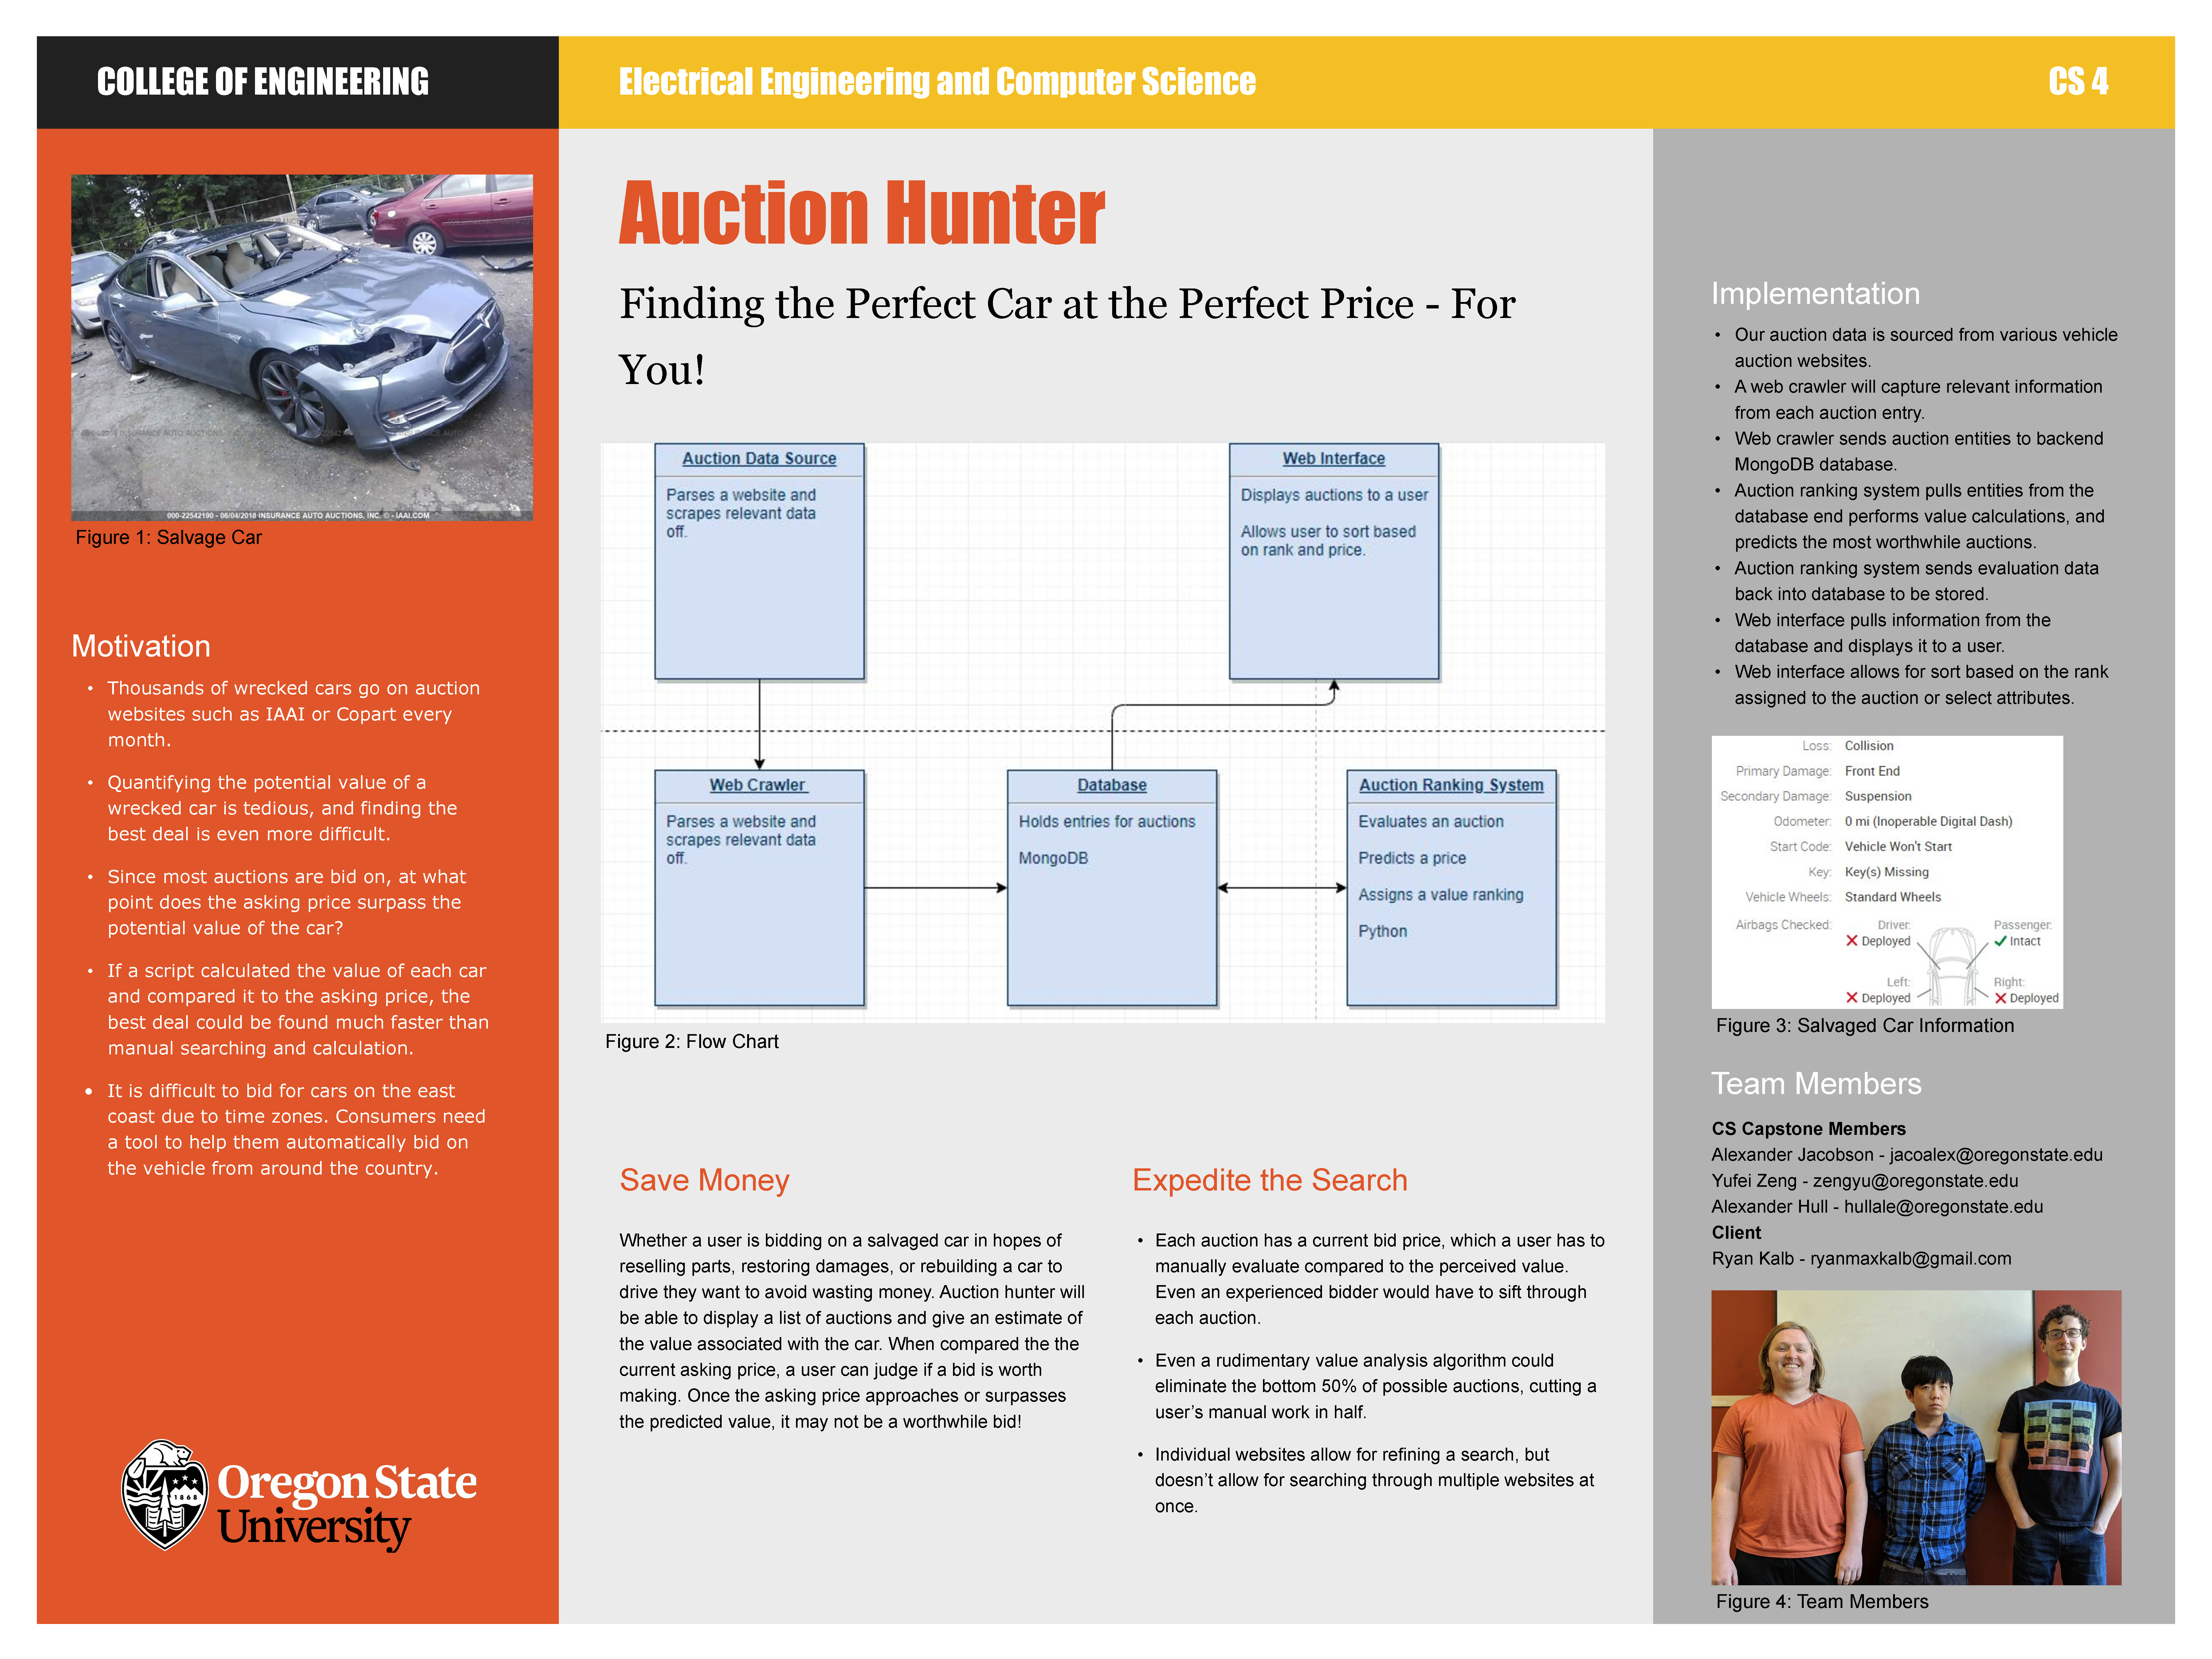
\includegraphics[width=\textwidth,keepaspectratio]{Poster.pdf}
    \caption{Poster}
    \label{fig:my_label}
\end{figure}


\section{Project Documentation}
\subsection{Project Layout}
\begin{figure}[ht]
    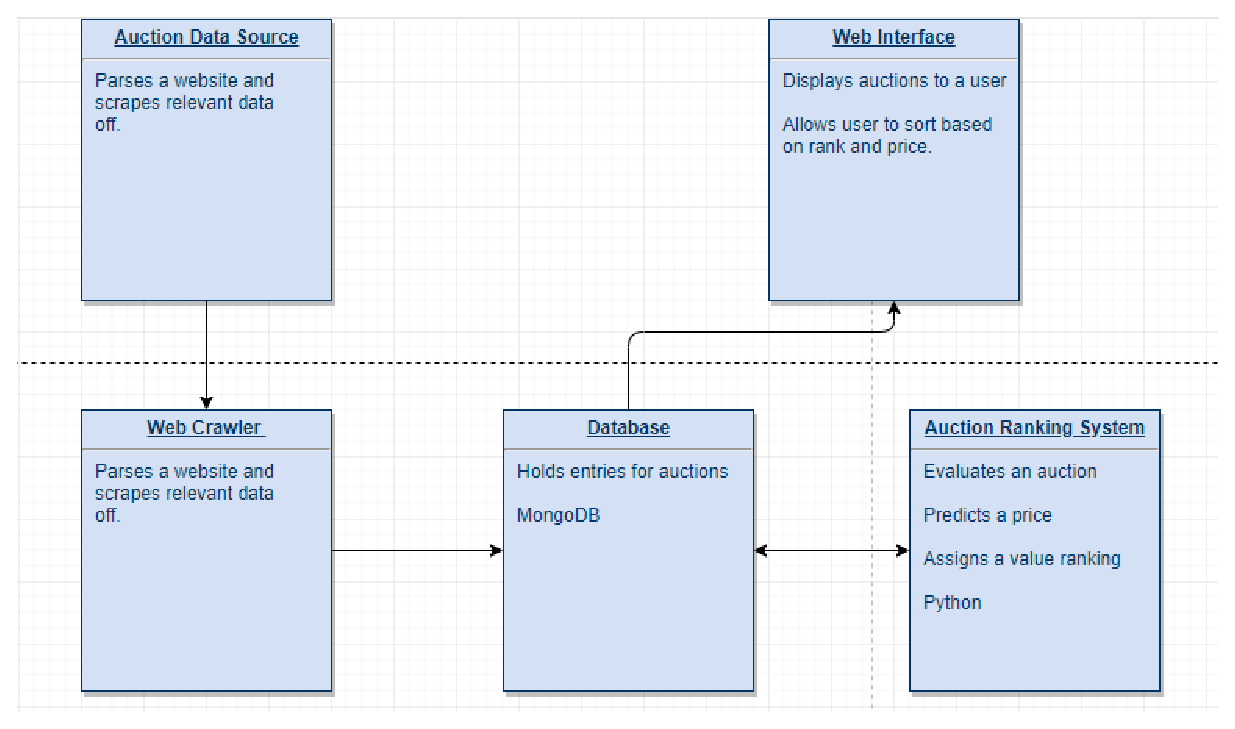
\includegraphics[scale=0.75]{flow_capture}
    \caption{Flow Design}
    \label{fig:flow}
\end{figure}
There are three key pieces to Auction Hunter: front-end, back-end, and scraper. The front end is what gets displayed to the user. This was written using React and JavaScript. This contects to the backend via REST endpoints exposed by the backend. This backend is a combination of a MongoDB database and a Python library called Django. The last piece is the scraper, also written in Python, scrapes the front ends of Auction Sites to gather data. For more detail look at the following diagram.

\subsection{Installation Guide}
The most up to date installation guide can be found in the README file in our  \href{https://github.com/AuctionHunter/AuctionHunter}{Github Repo}. The pieces of software need to run Auction Hunter are Python + Django, + Scrapy, NodeJS + React, and MongoDB. Auction Hunter should run on nearly any platform as Python and NodeJS have been ported to nearly everything, however, Auction Hunter has only been tested and deployed on Ubuntu and Windows, so other OSes may have bugs.
\url{https://github.com/AuctionHunter/AuctionHunter}

\section{Recommended Resources}
\begin{itemize}
    \item Django Documentation: \url{https://docs.djangoproject.com/en/2.2/}
    \item Django Rest Framework Documentation: \url{https://www.django-rest-framework.org/}
    \item React Documentation: \url{https://reactjs.org/docs/getting-started.html}
    \item Scrapy Documentation: \url{https://docs.scrapy.org/en/latest/intro/tutorial.html}
    \item MongoDB Documentation: \url{https://docs.mongodb.com/manual/}
\end{itemize}

\section{Conclusions and Reflections}
\subsection{Alexander Hull}
I was able to learn more about how to work with MongoDB with python. I also learned the basics of web scraping using Scrapy. I learned that there is a lot more to putting together a large project than just coding it. Establishing requirements and technologies is important. Its also a good idea to check in with the current status and the requirements along the way, to make sure the client is aware of the trajectory, and how it matches with the requirements. 

In regard to project work, I realized that maintaining a thread of communication between the team members and the client. Having everyone up to date is crucial to be able to collaborate effectively. It's difficult to be in a situation where everyone is self managing. Its a lot easier to have one person oversee the status of the project to keep things moving. 

If I were to repeat this project, I would make sure to lot get too lofty with out goals, and also communicate more effectively with my client. 
\subsection{Alexander Jacobson}
With this project I took a bit of what I already knew and expanded on it. I was familiar with Django and JavaScript frameworks, but for this project I taught myself React which is an extensive and quite large JavaScript web framework. 

Working together on a team can be quite challenging especially when learning new technologies and the most important thing I learned was to set reasonable and actionable goals each week of the project. This, I have found, keeps the project from overwhelming the team as well as making sure everyone is working on something that pushes the team towards completing the requirements. Its very easy for team members to all start working on different parts that might not come together to meet the initial goals.

If I were to do something different, I think it would be to have set more milestones along the way to make sure we all were making progress.

\subsection{Yufei Zeng}
Through this project, I learned a lot from both technical information and non-technical information. I learned the basics of web scraping base on Python frame. I was able to scrape the basic elements from any specific website and store them to local or cloud. In addition, I learned the basic of how web crawler Scrapy and MongoDB interact. 

Keeping good communication with the team members is essential to promote the progress of project. Weekly group meeting and weekly meeting with TA ensures that everyone will contribute something new for the project.

If I were to do something different for this project, I will communicate more with client, and satisfy client's requirements as more as possible.
\end{document}